\section{Case Study Results} \label{sec:casestudyresults}
In this section, we evaluate our approaches by answering two research questions. %For each research question, we present the motivation of the question, our approach to addressing the question and its corresponding results.

\subsection*{RQ1: How well can we model system performance under varying workloads?}

\subsubsection*{Motivation}
In order to use black-box machine learning models to detect performance regressions under varying workloads, we first need to understand whether such black-box models could accurately model the performance of a software system under varying workloads. %relationship between the runtime activities of a system (i.e., as recorded in logs) and its performance.
%The result of our approach highly depend on how well we model the system performance under varies workloads. 
Although prior research demonstrates promising results of using black-box models to capture the relationship between system performance and logs~\cite{Yao:2018:LSL:3184407.3184416,DBLP:conf/issre/FarshchiSWG15},
%for performance\ian{cite}\heng{seems only two papers model the realtionship between permance and logs~\cite{Yao:2018:LSL:3184407.3184416,DBLP:conf/issre/FarshchiSWG15}}, 
these models are built on predefined in-house workloads instead of varying field workloads. 
If such black-box models are sensitive to the variance in the workloads, they may not be suitable for modeling the performance of software systems under the field workloads from real end users.

% \vspace{-0.3cm}
\subsubsection*{Approach}
%\noindent\emph{Approach}
%To evaluate the models, we use prediction errors that are calculated by applying the models on the run-time data of the system. 
In order to understand the black-box models' ability for modeling system performance under varying workloads, we train the models on one set of workloads and evaluate the performance of the models on a different set of workloads (i.e., \emph{unseen} workloads).

%\smallskip
% \vspace{0.2cm}
\noindent\textbf{Modeling for the open source systems. }
For each open source system (i.e., OpenMRS and Apache James), we select the version of the system that is without performance regressions. We first run the system with four different concurrent workloads (i.e., \emph{4W}) and collect the logs and performance metrics. In order to ensure having new workloads to the system, we conduct another run by having an additional concurrent workload, i.e., having five different concurrent workloads (i.e., \emph{5W}). We build the performance models using the data that is generated by running the \emph{4W} workloads and apply the model on the data that is generated by running the \emph{5W} workloads. 
%We calculate the prediction error for each data point in the data is generated by having five different concurrent workloads. 
We evaluate the prediction performance of the black-box models on the 5W workloads by comparing the predicted performance and the measured performance.

%\smallskip

%\heng{Shall we first mention and put more focus on the industry system? Because we are talking about ``field workloads'' and we only use field workloads for the industry system.}
\noindent\textbf{Modeling for the industry system. }
For System X, we directly use the field data that is generated by workloads from the real end users. For each release cycle with $n$ days, we use the data from the first $n/2$ days to build the models and apply them on the data from the second $n/2$ days to evaluate the prediction performance of the models. We would like to note that there exists no control on the end users for applying any particular workload, and that all the data is directly retrieved from the field with no interference on the behavior of the end users. 
%Similar to the open source systems, the baseline prediction errors are calculated by applying 10-fold cross validation on the model and and data from the first $n/2$ days. 

\noindent\textbf{Analysis of modeling results. }
We calculate the prediction errors of the models on the new workloads (i.e., the \emph{5W} workloads for the open source systems and the second $n/2$-day workloads for System X).
In order to understand the magnitude of the prediction errors, we use the prediction errors of the models on the old workloads (i.e., the $4W$ workloads for the open source systems and the first $n/2$-day workloads for System X) as baselines. The baseline prediction errors are calculated using a 10-fold cross validation to avoid the bias of having the same training and testing data.  
\begin{itemize}
    \item \textbf{Median relative error}. The difference between the predicted performance and the measured performance, normalized by the measured performance.
    \item \textbf{p-value} (Mann-Whitney U). In order to understand whether the models trained on the old workloads can equivalently capture the system performance under the new workloads, we use the Mann-Whitney U test~\cite{nachar2008mann} to determine whether there exists a statistically significant difference (i.e., p-value $<$ 0.05) between the prediction errors on the new workloads and the prediction errors on the old workloads. %between being with and without a new workload.
    \item \textbf{Effect size} (Cliff\textquotesingle s delta). Reporting only the statistical significance may lead to erroneous results (i.e., if the sample size is very large, the p-value can be very small even if the difference is trivial)~\cite{sullivan2012using}. Therefore, we apply Cliff\textquotesingle s Delta~\cite{cliff1996ordinal} to quantify the effect size of the difference between the prediction errors on the old workloads and the prediction errors on the new workloads. 
    %The smaller the effect sizes, the more similar the prediction error between being with and without a new workload.
    %\heng{add the definition of trivial/small/median/large effect sizes}
\end{itemize}

\subsubsection*{Results}
Table \ref{tab:model_error} shows the detailed results of using six machine learning techniques to model the performance of the studied open source systems (i.e., \emph{OpenMRS} and \emph{Apache James}) under varying workloads.
 The column ``MRE'' shows the  median relative errors of applying the models (trained on the \emph{4W} workloads) on the \emph{4W} workloads and the \emph{5W} workloads, respectively. 
  The columns ``p-value'' and ``effect size'' show the statistical significance and the effect size of the difference between the prediction errors of the models on the \emph{4W} workloads and the prediction errors of the models on the \emph{5W} workloads, respectively. The ``violin plot'' column shows the distribution of the relative prediction errors under the \emph{4W} and \emph{5W} workloads.
% Moved the following description about the tables to the table title.
%The first column is a kind of performance model. The second column "Median relative error" consists of two sub columns. The first sub column indicates the number of concurrent workloads the system is running with, which can be either 4 workloads (4W) or 5 workloads (5W). The following sub column shows the corresponding prediction median relative error. The third column "P-value" shows the results of the statistical test on the two prediction error distribution of the system under different workloads. The column "Effect size" quantifies the difference of the prediction performance. The "Box plot" column includes the box plot of the prediction error distribution for different workloads. 

\begin{landscape}

\begin{table*}[htbp]
  \centering
%   \vspace{-0.3cm}
  \footnotesize
  \caption{Prediction error details for OpenMRS and Apache James under different workloads. 
%   \vspace{-0.2cm}
  %The first column is a kind of performance model.
 }
    
    \resizebox{.66\paperheight}{!}{
    \begin{tabular}{|c|c|c|c|c|c|c|c|c|c|c|}
    \hline
    \multirow{2}[4]{*}{Model} & \multicolumn{5}{c|}{OpenMRS}          & \multicolumn{5}{c|}{Apache James} \\
\cline{2-11}          & \multicolumn{2}{c|}{MRE} & P-value & Effect size & Violin plot & \multicolumn{2}{c|}{MRE} & P-value & Effect size & Violin plot \\
    \hline
    \multicolumn{1}{|c|}{\multirow{2}[9]{*}{Linear 
Regression}} & \multirow{1}[5]{*}{4W}    & \multirow{1}[5]{*}{3.12\%} & \multirow{2}[9]{*}{\textless 0.01} & \multirow{1}[10]{*}{-0.08} & \multirow{2}[4]{*}{ {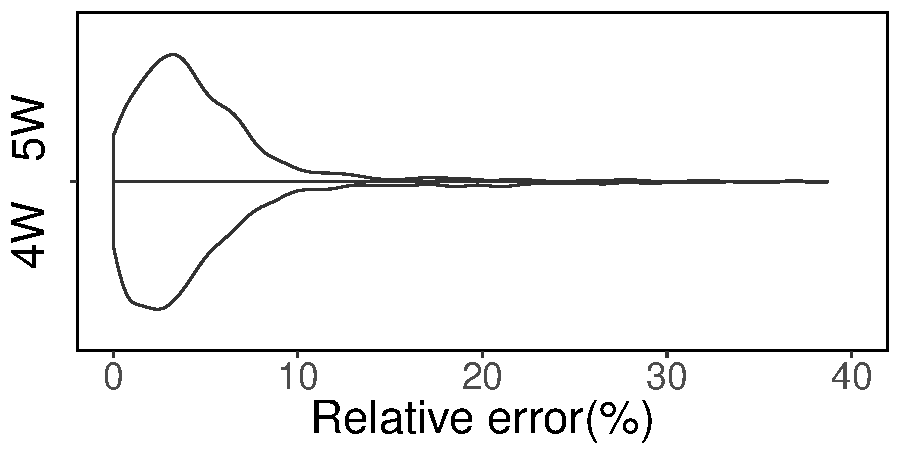
\includegraphics[height=15mm,width=30mm]{tex/figure/rq1/openmrs_linear_regression.pdf}}} & \multirow{1}[5]{*}{4W}    & \multirow{1}[5]{*}{23.24\%} & \multirow{2}[9]{*}{0.41} & \multicolumn{1}{c|}{\multirow{2}[9]{*}{N/A}} & \multirow{2}[4]{*}{{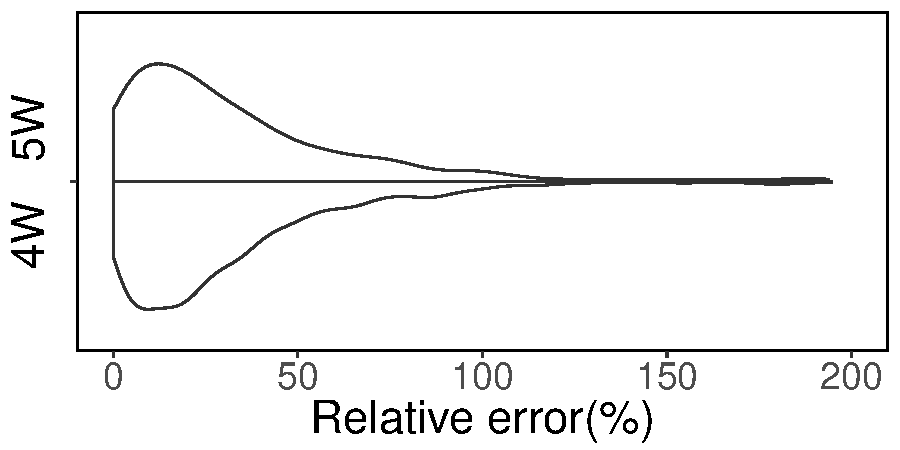
\includegraphics[height=15mm,width=30mm]{tex/figure/rq1/jms_linear_regression.pdf}}} \\[4.5mm]
\cline{2-3}\cline{7-8}          & \multirow{1}[5]{*}{5W}    & \multirow{1}[5]{*}{3.58\%} &       & (negligible) &       & \multirow{1}[5]{*}{5W}    & \multirow{1}[5]{*}{23.76\%} &       &       &  \\[4.5mm]
    \hline
    \multicolumn{1}{|c|}{\multirow{2}[9]{*}{Random 
Forest}} & \multirow{1}[5]{*}{4W}    & \multirow{1}[5]{*}{2.36\%} & \multirow{2}[9]{*}{\textless 0.01} & \multirow{1}[10]{*}{-0.09} & \multirow{2}[4]{*}{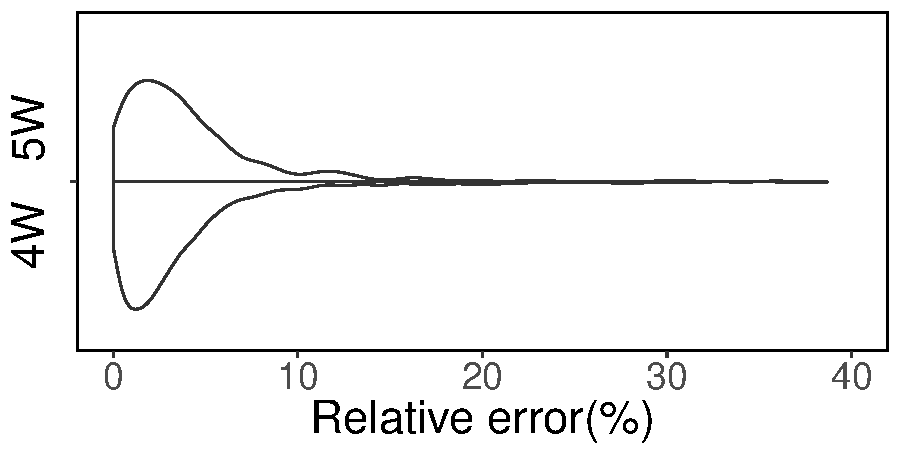
\includegraphics[height=15mm,width=30mm]{tex/figure/rq1/openmrs_random_forest.pdf}} & \multirow{1}[5]{*}{4W}    & \multirow{1}[5]{*}{22.99\%} & \multirow{2}[9]{*}{0.42} & \multicolumn{1}{c|}{\multirow{2}[9]{*}{N/A}} & \multirow{2}[4]{*}{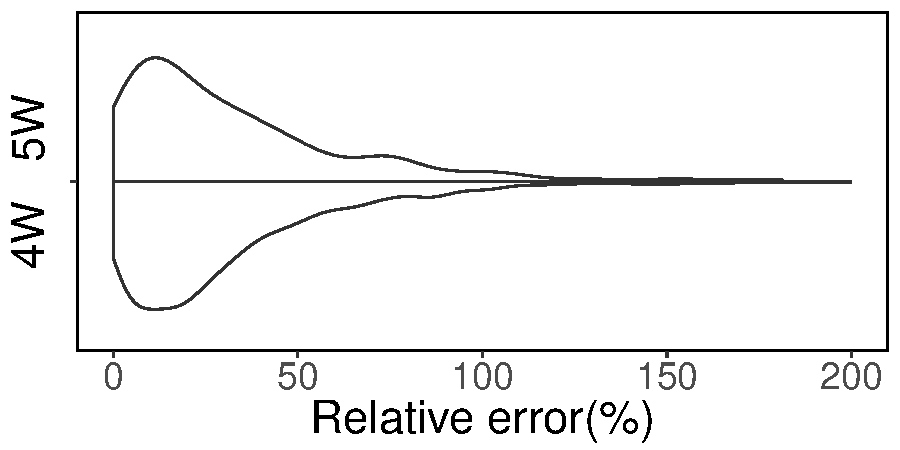
\includegraphics[height=15mm,width=30mm]{tex/figure/rq1/jms_random_forest.pdf}} \\[4.5mm]
\cline{2-3}\cline{7-8}          & \multirow{1}[5]{*}{5W}    & \multirow{1}[5]{*}{2.90\%} &       & (negligible) &       & \multirow{1}[5]{*}{5W}    & \multirow{1}[5]{*}{23.08\%} &       &       &  \\[4.5mm]
    \hline
    \multirow{2}[9]{*}{XGBoost} & \multirow{1}[5]{*}{4W}    & \multirow{1}[5]{*}{2.16\%} & \multirow{2}[9]{*}{0.14} & \multirow{2}[9]{*}{N/A} & \multirow{2}[4]{*}{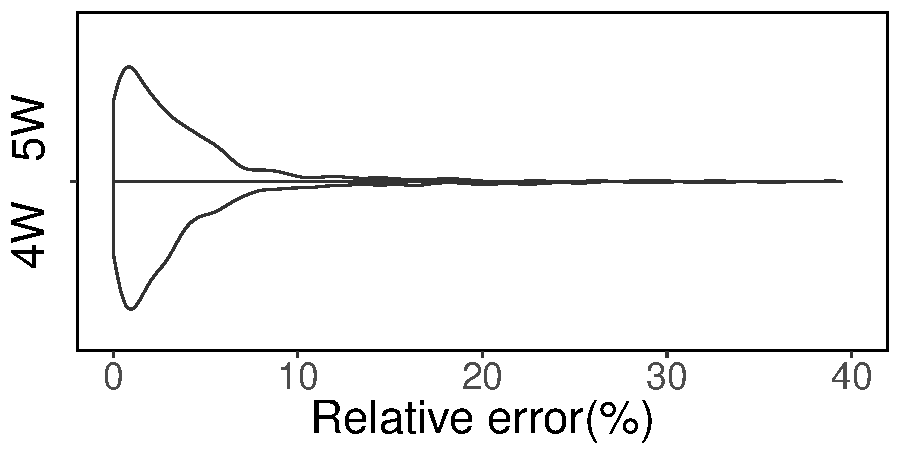
\includegraphics[height=15mm,width=30mm]{tex/figure/rq1/openmrs_xgboost.pdf}} & \multirow{1}[5]{*}{4W}    & \multirow{1}[5]{*}{24.29\%} & \multirow{2}[9]{*}{0.44} & \multirow{2}[9]{*}{N/A} & \multirow{2}[4]{*}{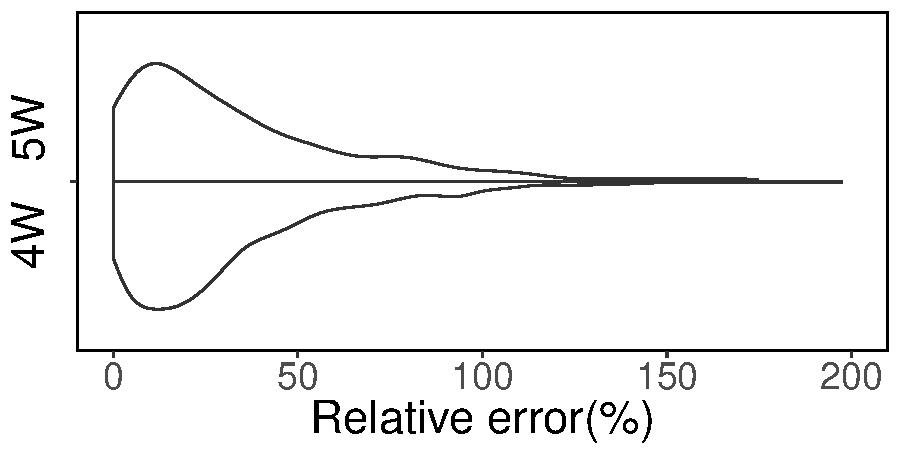
\includegraphics[height=15mm,width=30mm]{tex/figure/rq1/jms_xgboost.pdf}} \\[4.5mm]
\cline{2-3}\cline{7-8}          & \multirow{1}[5]{*}{5W}    & \multirow{1}[5]{*}{2.11\%} &       &       &       & \multirow{1}[5]{*}{5W}    & \multirow{1}[5]{*}{24.42\%} &       &       &  \\[4.5mm]
    \hline
    \multirow{2}[9]{*}{CNN} & \multirow{1}[5]{*}{4W}    & \multirow{1}[5]{*}{9.56\%} & \multirow{2}[9]{*}{\textless 0.01} & \multirow{1}[10]{*}{0.12} & \multirow{2}[4]{*}{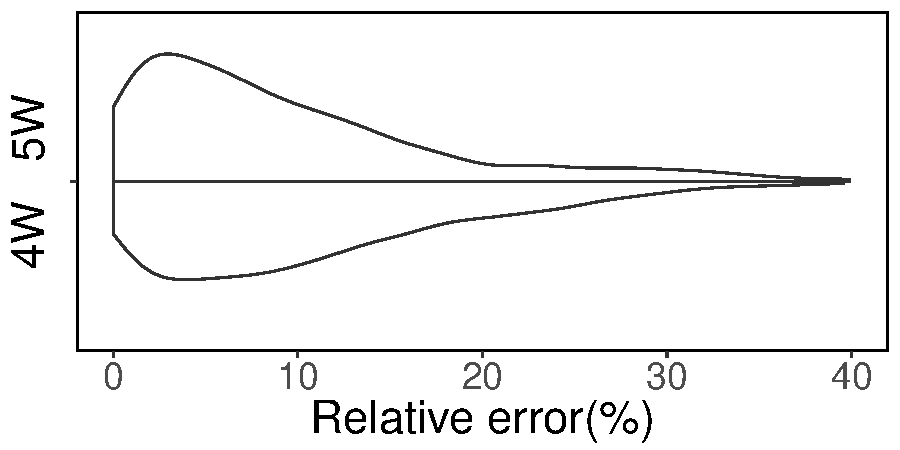
\includegraphics[height=15mm,width=30mm]{tex/figure/rq1/openmrs_cnn.pdf}} & \multirow{1}[5]{*}{4W}    & \multirow{1}[5]{*}{33.61\%} & \multirow{2}[9]{*}{0.11} & \multicolumn{1}{c|}{\multirow{2}[9]{*}{N/A}} & \multirow{2}[4]{*}{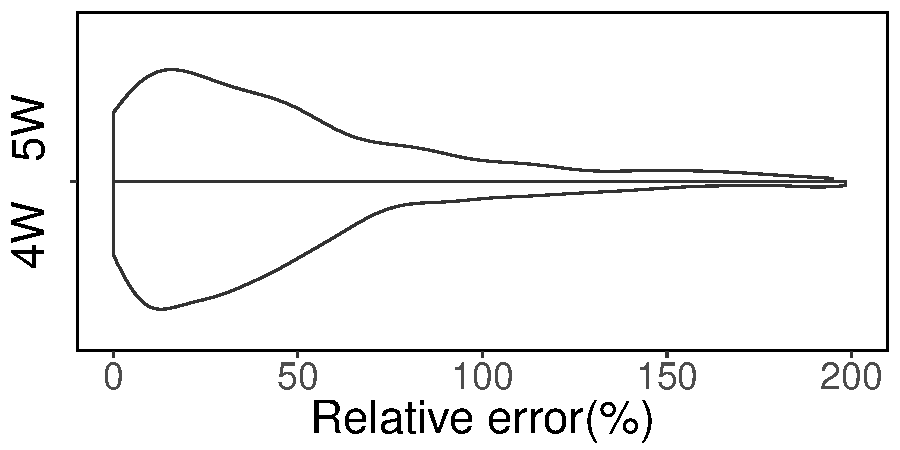
\includegraphics[height=15mm,width=30mm]{tex/figure/rq1/jms_cnn.pdf}} \\[4.5mm]
\cline{2-3}\cline{7-8}          & \multirow{1}[5]{*}{5W}    & \multirow{1}[5]{*}{7.47\%} &       & (negligible) &       & \multirow{1}[5]{*}{5W}    & \multirow{1}[5]{*}{37.51\%} &       &       &  \\[4.5mm]
    \hline
    \multirow{2}[9]{*}{RNN} & \multirow{1}[5]{*}{4W}    & \multirow{1}[5]{*}{5.63\%} & \multirow{2}[9]{*}{0.32} & \multirow{2}[9]{*}{N/A} & \multirow{2}[4]{*}{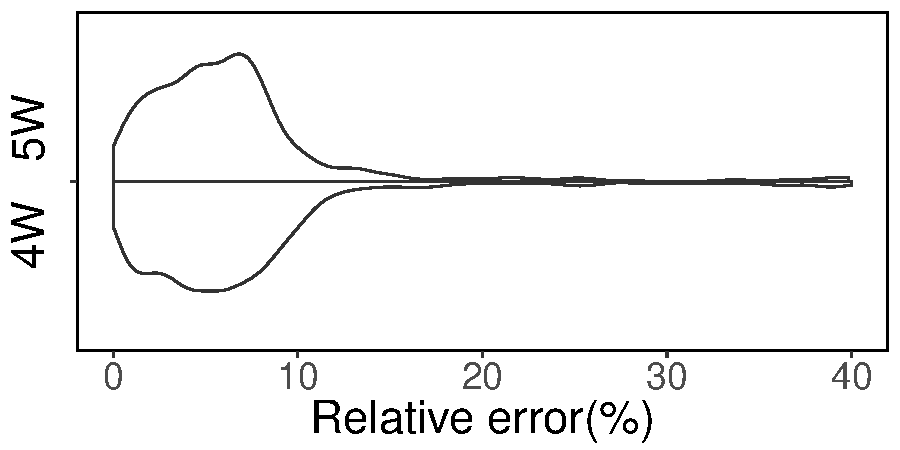
\includegraphics[height=15mm,width=30mm]{tex/figure/rq1/openmrs_rnn.pdf}} & \multirow{1}[5]{*}{4W}    & \multirow{1}[5]{*}{51.34\%} & \multirow{2}[9]{*}{0.01} & \multirow{1}[10]{*}{0.07} & \multirow{2}[4]{*}{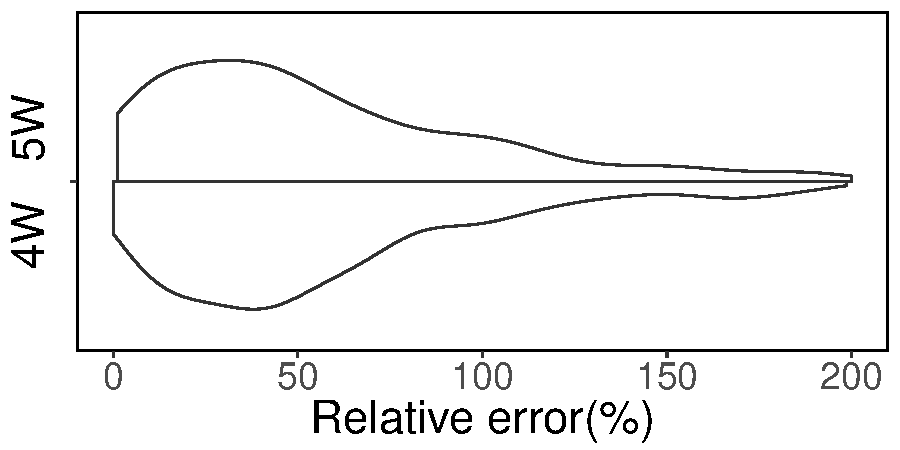
\includegraphics[height=15mm,width=30mm]{tex/figure/rq1/jms_rnn.pdf}} \\[4.5mm]
\cline{2-3}\cline{7-8}          & \multirow{1}[5]{*}{5W}    & \multirow{1}[5]{*}{5.73\%} &       &       &       & \multirow{1}[5]{*}{5W}    & \multirow{1}[5]{*}{47.22\%} &       & (negligible) &  \\[4.5mm]
    \hline
    \multirow{2}[9]{*}{LSTM} & \multirow{1}[5]{*}{4W}    &\multirow{1}[5]{*}{ 4.53\%} & \multirow{2}[9]{*}{\textless 0.01} & \multirow{1}[10]{*}{-0.25} & \multirow{2}[4]{*}{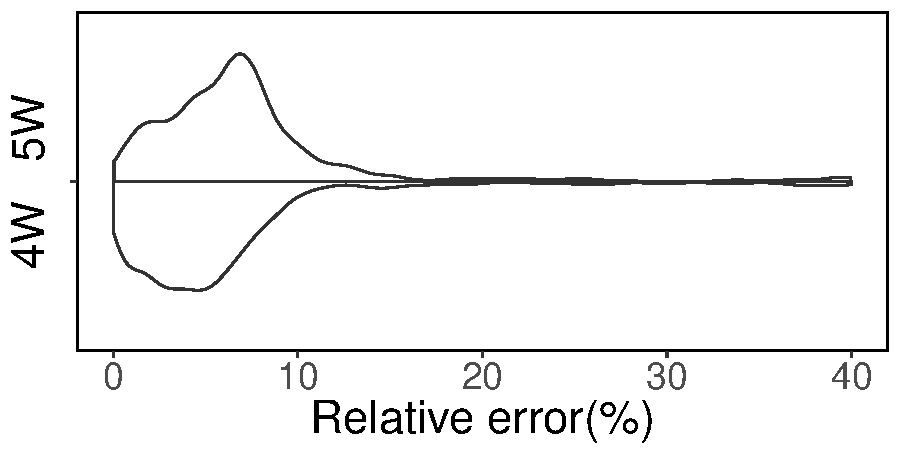
\includegraphics[height=15mm,width=30mm]{tex/figure/rq1/openmrs_lstm.pdf}} & \multirow{1}[5]{*}{4W}    & \multirow{1}[5]{*}{34.88\%} & \multirow{2}[9]{*}{\textless 0.01} & \multirow{1}[10]{*}{-0.27} & \multirow{2}[4]{*}{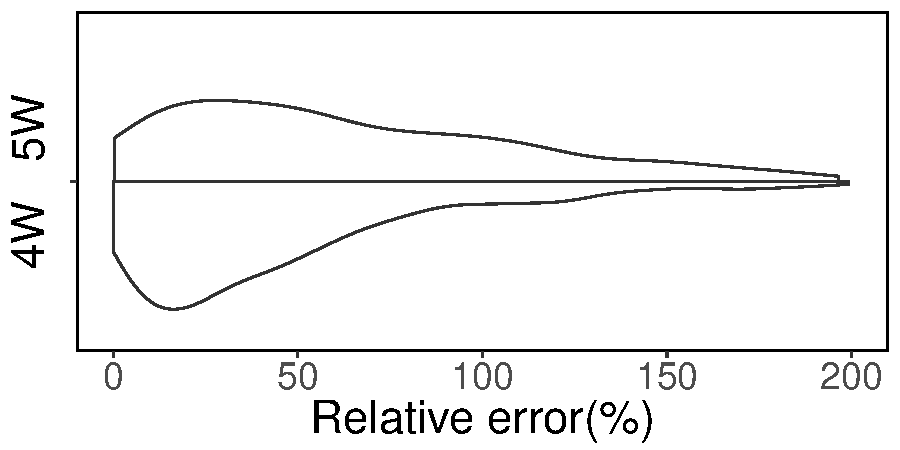
\includegraphics[height=15mm,width=30mm]{tex/figure/rq1/jms_lstm.pdf}} \\[4.5mm]
\cline{2-3}\cline{7-8}          & \multirow{1}[5]{*}{5W}    & \multirow{1}[5]{*}{6.42\%} &       & (small) &       & \multirow{1}[5]{*}{5W}    & \multirow{1}[5]{*}{57.11\%} &       & (small) &  \\[4.5mm]
    \hline
    \end{tabular}\\}
    Note: The column ``MRE'' presents the median relative errors.\hfill
  \label{tab:model_error}%
%   \vspace{-0.3cm}
\end{table*}%
\end{landscape}

\noindent\textbf{
%The performance prediction error of our models is diverse in different systems.
Our black-box models can accurately model the performance of the studied systems using the dynamic runtime activities that are recorded in the logs.} 
As shown in Table \ref{tab:model_error}, the XGBoost model achieves the best results for modeling the performance of the OpenMRS system, with a median relative error of 2.11\% on the \emph{5W} workloads (i.e., the new workloads) and a median relative error of 2.16\% on the \emph{4W} workloads (i.e., the baseline workload). 
The random forest model achieves the best results for Apache James, reaching a median relative error of 22.99\% and 23.08\% for the \emph{4W} workloads and \emph{5W} workloads, respectively. 
All the machine learning models achieve better results for the OpenMRS system than the results for the Apache James system.
The less-promising results for the Apache James system might be explained by the latency between the actual activities of the mail server system and the recorded logs. For example, the system can take an extended period of time to process an email with a large attachment, while a log about the successful processing of the email is only printed after the processing period.
%show that the best of our models is random forest (XGBoost is the best in \emph{OpenMRS}. However, there is need to adjust complex parameters), which achieves the lowest median relative error of 2.90\% and 23.08\% in \emph{OpenMRS} and \emph{Apache James}, respectively. 
%When we compare the median relative error between the baseline, performing 10-fold cross validation on the 4 concurrent workloads (4W), and under variable workloads (5W), we find that the median relative error of baseline in random forest model is 2.36\% and 22.99\% in \emph{OpenMRS} and \emph{Apache James}, respectively. It means that our model can considerably predict performance deviations under variable workloads.
%the simpler traditional models (e.g., linear regression and random forest) have lower performance prediction median relative error than the complex models(e.g. XGBoost and Deep Learning models). 
%By looking closely at each model, we can see that, in the different systems, the models has different performance on capturing the relationship between the performance of a system and its dynamic activities. For example, by using random forest model and performing 10-fold cross validation on the 4 concurrent workloads on OpenMRS and Apache James, the median error relative error almost ten times (from 2.36\% to 22.99\%). However, in comparison to the rest models, the CNN model has the relatively lower difference on the prediction performance, which the MRE in Apache James is around 3.5 times the MRE in OpenMRS.

\noindent\textbf{The traditional models (e.g., linear regression and random forest) outperform the deep neural networks (e.g., CNN and RNN) for modeling the performance of the studied systems.}
As shown in Table~\ref{tab:model_error}, for both the OpenMRS and the Apache James systems, the three traditional models achieve better results than the three deep neural networks for modeling the system performance.
These results indicate that the relationship between the system performance and the runtime activities recorded in the logs can be effectively captured by the simple traditional models.
Such results also agree with a recent study~\cite{DacremaArxiv2019} that compares deep neural networks and traditional models for the application of automated recommendations.


%\textbf{Our models perform well in terms of robustness and stability.}
\noindent\textbf{Our black-box models can equivalently explain the performance of a system under new workloads that are unseen when constructing the models.}
%\heng{To be revised.}
%In order to understand whether our black-models built on the old workloads (e.g., the \emph{4W} workloads) can model the system performance under the new workloads (e.g., the \emph{5W} workloads), 
Table~\ref{tab:model_error} shows the statistical significance (i.e. the p-value) and the effect size of the difference between the prediction errors of applying the old models (i.e., trained from the \emph{4W} workloads) on the new workloads (i.e., the \emph{5W} workloads) and applying the old models on the old workloads (i.e., the \emph{4W} workloads). 
Table \ref{tab:model_error} also compares the distributions of the prediction errors for the \emph{4W} and \emph{5W} workloads.
The prediction errors of most of the models (except LSTM) have either statistically insignificant or negligible difference between the \emph{4W} and the \emph{5W} workloads, indicating that the models trained from the old workloads can equivalently model the system performance under new workloads.
The LSTM model results in a \emph{small} difference of the predictions errors between the \emph{4W} and the \emph{5W} workloads. We suspect that the complex LSTM model is likely over-fit towards the training workloads.
%When conducting the statistical tests into the prediction error between being with and without a new workload, in the total of 6 models, we find that there are 4 and 2 models in \emph{OpenMRS} and \emph{Apache James} have statistically significantly difference on the distribution of the performance prediction error. However, when we quantify the difference, we find that the effect sizes among these models are either negligible (4) or small (2). Such results imply that our models perform stably under variable workloads.
%The distribution of the performance prediction error of our models is consistent when the system is under different workloads. In total, we have used 6 models that includes traditional models, machine learning models and deep learning models to capture the the relationship between the performance of a system and its dynamic activities that are recorded in logs. 
%When conducting the statistical tests to determine whether there exists a statistically significant difference between prediction error between being with and without a new workload. If the P-value greater than 0.05, it mean there is no statistically significant difference; whereas when the P-value smaller than 0.05, we further calculate the effect size to check how much the difference is. In the Table \ref{tab:openmrs_error}, we can see that four models in OpenMRS have P-value smaller than 0.05, among these model, only the LSTM has a small effect size and the rest is negligible. Table \ref{tab:jms_error} shows, in the Apache James, four models perform the same when adding one new workload to the existing four workloads and the reset two have one negligible and one small effect size. 

%Discussion: \textbf{Traditional machine learning models (e.g., linear regression and random forest) perform better than than deep learning models (e.g., LSTM).}

%\heng{Shall we talk a little bit about the industry system.}

Due to an NDA, the detailed results of using the machine learning techniques to model the performance of the industry system (i.e, System X) are not presented in this paper. However, the results are similar to the shown results for the open source systems. In particular, when modeling the performance of all 10 studied versions of System X, the prediction errors are all between 10\% to 20\%. In addition, when we evaluate the models with different workloads, the differences between prediction errors are all either statistically insignificant or with negligible/small effect sizes.



\hypobox{Simple traditional models (e.g., linear regression and random forest) can accurately capture the relationship between the performance of a system and its dynamic activities that are recorded in logs, with varying workloads.
%, achieving a median relative error of 2.11\% to 3.58\% for OpenMRS and 22.99\% to 24.42\% for Apache James.
%In addition, such models can equivalently capture the performance of a system under new workloads that are unseen when constructing the models.
}

\subsection*{RQ2: Can our approach detect performance regressions under varying workloads?}

\subsubsection*{Motivation}

In traditional performance testing, in order to detect performance regressions, performance analysts compare the performance data of two versions of a software system that is generated by running the same workloads from the same performance test suites. 
However, in a field environment, as the workloads of the systems are constantly changing, it is almost impossible to run two software versions on the same workloads to detect performance regressions.
The results of RQ1 show that our black-box models can accurately capture the performance of a software system even under new workloads that are unseen when training the models.
%The results of RQ1 shows that having new workloads may lead to higher prediction errors of the black-box performance models. Although the magnitude of the difference is either statistically insignificant, negligible, or small, it may still brings noise to the detection of performance deviance, causing potential false results of our approach. 
Therefore, in this research question, we would like to leverage such black-box models to detect performance regressions when the workloads of the two versions of a system are not consistent.

Running the systems for hours or days before discovering performance regressions incurs a high cost. As the systems are already running in the field, any delay in detecting the performance regressions may pose huge impact on the end users. Hence, a desired approach in practice should be able to detect performance regression in a timely manner. Therefore, we also want to study how fast our approaches can detect performance regressions. 

\subsubsection*{Approach}

The results from RQ1 show that random forest and XGBoost have the lowest prediction errors when modeling performance (cf. Table~\ref{tab:model_error}). Since XGBoost requires resource-heavy fine-tuning, we opt to use random forest in this research question. For the open source systems, we first build the performance models from running the systems without performance regressions under the \emph{4W} workloads (i.e., a combination of four different concurrent workloads). We then run the systems without performance regressions under the \emph{5W} workloads (i.e., a combination of five different concurrent workloads). Ideally, our approach should not detect performance regressions from these runs. 
We use such results as a baseline to evaluate the effectiveness of our approach for detecting performance regressions under the new workloads (i.e., the \emph{5W} workloads). 
Afterwards, we run the systems with the performance regressions (cf. Table~\ref{tab:workloaddeisign}) under the \emph{5W} workloads. Our approach should be able to detect performance regressions from these runs.

For the System X from the industry, for every new release, we use our approach to compare the field data from the new release and the previous release to determine whether there are performance regressions. Since there are no injected or pre-known performance regressions, we present the detected performance deviance to the developers of the systems and manually study the code changes to understand whether the detection results are correct. For the releases that are detected as not having performance regressions, we cannot guarantee that these releases are free of performance regressions. However, we also present the results to the developers to confirm whether there exist any users who report performance-related issues for these releases. If so, our detection results may be considered false.

Finally, to study how fast our approaches can detect performance regressions, for the new versions of the systems that have performance regressions, we only use the first 15-minute data and apply our approach to detect the performance regressions. Then, we follow an iterative approach to add another 5-minute data to the existing data, until our approach can detect the performance regressions (i.e., with a medium or large effect size that is higher than the baseline). %\heng{to revisit to make it more clear}.

\subsubsection*{Results}

\noindent\textbf{Our black-box-based approaches can effectively detect performance regressions under varying workloads.}
% - The effect size of the difference between two versions can detect performance regressions
% - Effect size and threshold for OpenMRS, Apache James, and the industry system
Table~\ref{tab:predictionresult_rq2} shows the results of our three approaches of performance regression detection (cf. Section~\ref{sec:comparions-approaches}) on OpenMRS and Apache James. We find that with all three approaches, when there are known performance regressions between two versions, the statistical analysis always shows significant difference between the two versions with medium or large effect sizes. In addition, the effects sizes from Approach 1 and 2 are negative, confirming the existence of performance regressions (negative values indicate performance regression and positive values indicate performance improvement). 

When we compare the effect sizes with the baseline, i.e., running our approaches with systems without performance regressions but under two different workloads, we find that the baseline effect sizes are always smaller than the corresponding ones with performance regressions, except when detecting the regression in v3 of OpenMRS. We consider the reason being the nature of the regression in v3, i.e., an injected delay. Since our considered performance metric is the CPU usage and such a delay may not have large impact on the CPU usage, it is difficult for our approaches to detect such a regression. 

% Table generated by Excel2LaTeX from sheet 'Sheet1'

\begin{table}[tbh]
  \centering
%   \vspace{-0.3cm}
  \tiny
  \tabcolsep=0.14cm
  \caption{Performance regression detection results for OpenMRS and Apache James. }
%   \vspace{-0.2cm}
    \begin{tabular}{|c|c|c|c|c|c|c|c|}
    \hline
    \multicolumn{8}{|c|}{OpenMRS} \\
    \hline
    \multicolumn{2}{|c|}{Versions} & \multicolumn{2}{c|}{Approach 1} & \multicolumn{2}{c|}{Approach 2} & \multicolumn{2}{c|}{Approach 3} \\
    \hline
    \multicolumn{1}{|p{0.7cm}<{\centering}|}{Old\newline{}version} & \multicolumn{1}{|p{0.7cm}<{\centering}|}{New\newline{}version} & \multirow{1}[3]{*}{P-value} & \multirow{1}[3]{*}{Effect size} & \multirow{1}[3]{*}{P-value} & \multirow{1}[3]{*}{Effect size} & \multirow{1}[3]{*}{P-value} & \multirow{1}[3]{*}{Effect size} \\
    \hline
    v0 & v0 & \ll0.001 & 0.39 (medium) &  \ll0.001 & 0.36 (medium) & \ll0.001 & 0.17(small) \\
    \hline
    v0 & v1 & \ll0.001 & -0.59 (large) & \ll0.001 & -0.69 (large) & \ll0.001 & 0.38 (medium) \\
    \hline
    v0 & v2 & \ll0.001 & -0.44 (medium) & \ll0.001 & -0.63 (large) & \ll0.001 & 0.37 (medium) \\
    \hline
    v0 & v3 & \ll0.001 & -0.36 (medium) & \ll0.001 & -0.42 (medium) & \ll0.001 & 0.53 (large) \\
    \hline
    v0 & v4 & \ll0.001 & -0.69 (large) & \ll0.001 & -0.76 (large) & \ll0.001 & 0.51 (large) \\
    \hline
%        \multicolumn{1}{r}{} & \multicolumn{1}{r}{} & \multicolumn{1}{r}{} & \multicolumn{1}{r}{} & \multicolumn{1}{r}{} & \multicolumn{1}{r}{} & \multicolumn{1}{r}{} & \multicolumn{1}{r}{} \\
    \hline
    \multicolumn{8}{|c|}{Apache James} \\
    \hline
    \multicolumn{2}{|c|}{Versions} & \multicolumn{2}{c|}{Approach 1} & \multicolumn{2}{c|}{Approach 2} & \multicolumn{2}{c|}{Approach 3} \\
    \hline
    \multicolumn{1}{|p{0.7cm}<{\centering}|}{Old \newline{}version} & \multicolumn{1}{|p{0.7cm}<{\centering}|}{New \newline{}version} & \multirow{1}[3]{*}{P-value} & \multirow{1}[3]{*}{Effect size} & \multirow{1}[3]{*}{P-value} & \multirow{1}[3]{*}{Effect size} & \multirow{1}[3]{*}{P-value} & \multirow{1}[3]{*}{Effect size} \\
    \hline
    3.0m2 & 3.0m2 & 0.008 & 0.09 (negligible) & \ll0.001 & -0.12 (negligible) & \ll0.001 & -0.03 (negligible) \\
    \hline
    3.0m2 & 3.0m1 & \ll0.001 & -0.65 (large) & \ll0.001 & -0.76 (large) & \ll0.001 & 0.41 (medium) \\
    \hline
    3.0m2 & 2.3.2 & \ll0.001 & -0.90 (large) &\ll0.001 & -0.93 (large) & \ll0.001 & 0.82 (large) \\
    \hline
    \end{tabular}\\
    Note: For all the old versions, we use four concurrent workloads and for all the new versions with and without regressions, we use five concurrent workloads (one extra workload).\hfill
  \label{tab:predictionresult_rq2}%
%   \vspace{-0.3cm}
\end{table}%

For all the 10 releases of System X, our approaches detected performance regressions from one release.
All three approaches detected performance regressions from the release with large effect sizes when compared with the previous release.
All three approaches did not detect performance regressions from the other nine releases (i.e., with either statistically insignificant difference or negligible effect sizes when compared with the previous release). 
By further investigating the release with performance regressions, we observed that developers added a synchronized operation to lock the resources that are responsible for generating a report, in order to protect the shared resources under the multi-thread situation. However, the reporting process is rather resource-heavy, resulting in significant overhead for each thread to wait and acquire the resources. Thus, the newly added lock causes the performance regression. After we discussed with the developers who are responsible for this module, we confirmed that this synchronized operation introduced performance regression to the software. 
In addition, for all the nine releases from which our approaches did not detect performance regressions, the developers of System X have not yet received any reported performance issues from the end users till the day of writing this paper.

%When comparing the predicted value and the actual value of performance metrics (Approach 1), and the prediction of performance metrics between using model built from the old version and the model build from the new version (Approach 2), we find that the predictions of runs with performance regression have all negative values (Positive/negative value means performance improvement/regression). In addition, we observe that the effect sizes of the difference between two versions are medium or large.

%In the approach of A3, we observe that the effect sizes of difference between prediction errors are negligible or small within runs without performance regression (v0-v0, 3.0m2-3.0m2), medium or large within runs with performance regression. Such results imply that all three approaches can successfully detect real and injected performance deviation under varying workloads automatically without manual setting threshold.

%The effect size of the difference between two versions can detect performance regressions. For approach 1 and approach 2, we compare the predictions based on model trained on the old version data with true value and predictions based on the model trained on the new version data. In both OpenMRS and Apache James, the runs with performance regression have all negative and larger effect size (except for approach 1, run v0-v3) than the run with out regression, which means the new version system has performance regression. For approach 3, we can see that the runs with performance regressions always has larger effect size than the runs without performance regressions. Thus, all the results show that our three black-box-based approach can effectively detect both real and injected performance regressions under varying workloads.

\noindent\textbf{Comparing the prediction errors is more effective than comparing the prediction values when detecting performance regressions between two versions.}
We observe that for OpenMRS, the differences between the prediction values using Approach 1 and 2 can still be medium (0.39 and 0.36) even for the baseline (i.e., without regressions).
On the other hand, when comparing the prediction errors instead of the prediction values, i.e, using Approach 3, the baseline without regressions has only a small effect size (0.17).
Such a smaller baseline effect size makes Approach 3 easier to be adopted in practice, i.e., without the need of spending efforts searching for an optimal threshold on the effect size to detect performance regressions. However, Approach 3 only shows the deviance of the prediction errors without showing the direction of the performance deviance, thus it cannot distinguish a performance regression from a performance improvement. Hence, Approach 3 may be used first to flag the performance deviance then be combined with other approaches in practice to determine whether the performance deviation is a performance regression or a performance improvement.


%In the approach A3, the effect sizes of predictions of the difference are negligible (-0.03) \emph{Apache James} and small (0.17) in \emph{OpemMRS}. Such results imply that although A1, A2 and A3 can detect performance deviation, Approach 3 is more reasonable and explanatory than Approach 1 and 2.
%However, in 2 out of 4 runs (v0-v2, v0-v3) with performance deviation in A1, 1 out of 4 runs (v0-v3) with performance deviation in A2, the effect sizes are also medium. 
%Such results require performance analysts to determine a specific threshold of effect size based on their experience or gut feeling. On the contrary, in approach A3, we find that the distance of effect size between the runs with performance deviation and baseline ranges from 0.2 (v0-v2) to 0.38 (3.0m2-3.0m1). Therefore, A3 outperforms A1 and A2 in detection of performance deviation.
%Our approach needs different settings of the effect size threshold for detecting real and injected performance regressions. }
% - Real performance regressions (Apache James and the industry system) need a lower threshold
% - Injected performance regressions (OpenMRS) need a higher threshold
%From Table \ref{tab:predictionresult_rq2}, we can see that for OpenMRS and Apache James, the threshold for determining whether there is the performance regression is different. In OpenMRS, among three approaches, the effect size of difference on the runs without performance regression is from 0.17 to 0.39, while in Apache James this number is from 0.03 to 0.12. Thus, real performance regression in Apache James and the industry system need a lower threshold, whereas injected performance regressions in OpenMRS need a higher threshold.


%\noindent\textbf{Calculating the effect size of the difference between the prediction errors of the old model and the prediction errors of the new model can detect performance regressions most effectively.}
% - Pros and cons of different methods
% - How they can be combined to detect performance regressions
%Table \ref{tab:predictionresult_rq2} shows the prediction result of our three approaches on OpenMRS and Apache James. Among these three approaches, the approach 3 always have most effective results on both systems, since it has the most clear effect size gap between runs with regression and runs without regression. However, there is a drawback of this approach, which is that although it can only tell us whether there is performance deviations between old version system and new version systems, it cannot tell it is performance regression or performance improvement. In order to detect performance regression, we also need to combine approach 3 with one of the other two approaches, since approach 1 and 2 have the ability to determining whether the performance deviation is belongs to performance regression or performance improvement. 
% The negative effect size shows the performance regression.



%\subsubsection*{Discussion}
%\noindent\textbf{Our approaches can detect performance regressions with as early as 15-minutes data.}
\noindent\textbf{Our approaches can detect performance regressions as early as 15 minutes after running a new version.}
Table~\ref{tab:howearly} shows the earliest time that our approach can detect performance regressions in the studied open source systems. We find that all the performance regressions in the open source systems can be detected by at least one approach with less than 20-minute data from the new version. In particular, the regressions from both versions of Apache James and three versions of OpenMRS can even be detected using only the first 15-minute data. The ability of early detection eases the adoption of our approaches in the practices of testing in the field, where performance regressions are detected directly based on the field data, instead of using dedicated performance testing. 
 
\begin{table}[tbh]
  \centering
%   \vspace{-0.2cm}
%   \footnotesize
  \caption{The earliest time for our approaches to detect regressions in the two open source systems.}
%   \vspace{-0.2cm}
    \begin{tabular}{c|cccc|cc}
    \hline
          & \multicolumn{4}{c|}{OpenMRS}  & \multicolumn{2}{c}{Apache James} \\
\cline{2-7}          & v1    & v2    & v3    & v4    & 3.0m1 & 2.3.2 \\
    \hline
    Approach 1 & 60 mins & 160 mins & 15 mins & 15 mins & 15 mins & 15 mins \\
    Approach 2 & 20 mins & 50 mins & 15 mins & 15 mins & 15 mins & 15 mins \\
    Approach 3 & 45 mins & 15 mins & 15 mins & 15 mins & 15 mins & 15 mins \\
    \hline
    \end{tabular}%
  \label{tab:howearly}%
%   \vspace{-0.3cm}
\end{table}%






\hypobox{All three approaches can successfully detect performance regression under varying workloads, requiring data from a very short period of time (down to 15 minutes). 
%The deviance of prediction errors is a more effective indicator than prediction values. 
Comparing the prediction errors is more effective than comparing the prediction values for detecting performance regressions between two versions.
}


